\documentclass[letterpaper,onecolumn,draftclsnofoot]{IEEEtran}
\usepackage{amsmath,amssymb,booktabs,graphicx,array}
\usepackage[hidelinks]{hyperref}
\renewcommand{\thetable}{S\arabic{table}}
\renewcommand{\thefigure}{S\arabic{figure}}
\newcommand{\D}{\mathcal{D}}
\newcommand{\W}{\mathcal{W}}
\begin{document}
\title{Supplementary Material: When Should Robots Hide Where They Wait?\\ Leakage-Aware Randomized Staging for Capacity-Constrained Multi-Robot Response}
\author{Syed Muhammad Alam and Hamza Rafique}
\maketitle

\section*{S0. Reproducibility protocol}
\textbf{Hardware and software.} One core of an Intel Xeon (2.1\,GHz) cloud machine; Python 3.13, NumPy 2.5, SciPy 1.18 (HiGHS), numba 0.68, networkx 3.x; Gazebo Harmonic 8.10, ROS~2 Jazzy, Nav2 (RoboStack conda-forge builds); Mesa llvmpipe for headless rendering. All solver timings are single-threaded wall-clock, excluding Python start-up and one-time numba compilation.

\textbf{Tolerances.} Constraint generation adds attacks while a violation exceeds $10^{-9}$ (relative); defender-side certificates and the $q^\star$ tie test use $10^{-7}$ (relative); $\D^\star=\{d:\mu_d\ge P-10^{-9}\}$; Charnes--Cooper scale cap $\lambda\le10^8$ (never active; largest non-tie $q^\star=0.993$); bisection on $V^\star(q)$ to $10^{-3}$ in the sensitivity study.

\textbf{Randomization and units.} Instance generators use NumPy PCG64 with seeds fixed in the scripts (grid: \texttt{instances.py}; maps: \texttt{sim.scenario}). In the closed-loop simulation every policy evaluated for a given (layout, $q$) uses the same seed (CRC32 of map, layout, regime and $q$) and the same per-shift uniforms (configuration draw by inverse CDF, attack time, surveillance) and per-robot-slot speed and success draws, so comparisons are paired. Shifts are nested in layouts; the layout (or map, in the grid) is the independent unit, and intervals are 95\% $t$-intervals over those units.

\textbf{Lemma 2 example.} Sites 1--4, $m=2$, $c=1$, $n=2$, $p=0.9$; zone $A$ ($v=10$) reachable from sites 1,2 and zone $B$ ($v=1$) from sites 3,4. Expected values under $x$ (\{1,2\} or \{3,4\}): $w=(2,0)\colon5.05$, $(1,1)\colon4.95$, $(0,2)\colon10.405$. Under $x'$ (\{1,3\} or \{2,4\}): $(2,0)\colon1.0$, $(1,1)\colon9.9$, $(0,2)\colon10.0$. Both open every site with probability $\tfrac12$; $z(x)=4.95$, $z(x')=1.0$ (file \texttt{lemma2\_example.json}).

\begin{figure}[h]\centering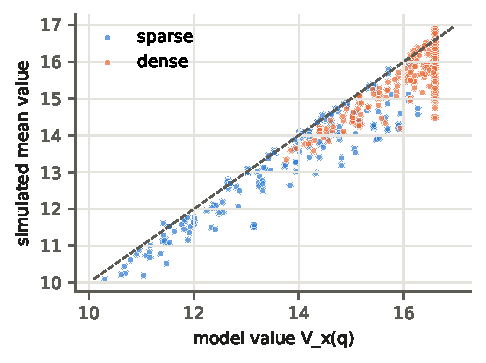
\includegraphics[width=0.55\textwidth]{fig_model_vs_sim.pdf}
\caption{Model value $V_x(q)$ versus simulated mean value for all 450 closed-loop runs ($r=0.955$; simulator 3.1\% lower on average). The dashed line marks equality.}\end{figure}

\begin{table}[h]\centering\caption{Closed-loop simulation, all policies (15 layouts; mean simulated value, change vs.\ fixed maximin with 95\% $t$-interval over layouts, layouts with a gain, relocation distance per shift, fraction of shifts observed).}\label{tab:s-sim}\scriptsize
\begin{tabular}{@{}llrrrrr@{}}\toprule regime & policy & $q$ & value & $\Delta$ vs fixed (\%) & wins & reloc.\ (m) / obs.\\\midrule
sparse & fixed maximin & 0.0 & 13.45 & $0.00\pm0.00$ & 0/15 & 0 / 0.000\\
sparse & mexclp & 0.0 & 13.34 & $-0.81\pm1.07$ & 0/15 & 0 / 0.000\\
sparse & uniform random & 0.0 & 11.78 & $-12.02\pm4.11$ & 1/15 & 110 / 0.002\\
sparse & concealed q0 & 0.0 & 14.51 & $8.09\pm2.67$ & 15/15 & 70 / 0.001\\
sparse & leakage aware & 0.0 & 14.51 & $8.09\pm2.67$ & 15/15 & 70 / 0.001\\
sparse & fixed maximin & 0.25 & 13.46 & $0.00\pm0.00$ & 0/15 & 0 / 0.255\\
sparse & mexclp & 0.25 & 13.36 & $-0.77\pm1.08$ & 0/15 & 0 / 0.255\\
sparse & uniform random & 0.25 & 11.33 & $-15.45\pm3.78$ & 0/15 & 110 / 0.257\\
sparse & concealed q0 & 0.25 & 14.02 & $4.32\pm2.47$ & 12/15 & 70 / 0.256\\
sparse & leakage aware & 0.25 & 14.21 & $5.76\pm2.31$ & 13/15 & 56 / 0.257\\
sparse & fixed maximin & 0.5 & 13.47 & $0.00\pm0.00$ & 0/15 & 0 / 0.503\\
sparse & mexclp & 0.5 & 13.35 & $-0.93\pm1.29$ & 0/15 & 0 / 0.503\\
sparse & uniform random & 0.5 & 10.95 & $-18.43\pm3.57$ & 0/15 & 111 / 0.503\\
sparse & concealed q0 & 0.5 & 13.58 & $0.95\pm2.41$ & 7/15 & 71 / 0.503\\
sparse & leakage aware & 0.5 & 13.80 & $2.57\pm2.06$ & 10/15 & 49 / 0.503\\
dense & fixed maximin & 0.0 & 15.59 & $0.00\pm0.00$ & 0/15 & 0 / 0.000\\
dense & mexclp & 0.0 & 15.76 & $1.25\pm2.73$ & 5/15 & 0 / 0.000\\
dense & uniform random & 0.0 & 15.02 & $-3.45\pm2.95$ & 3/15 & 111 / 0.002\\
dense & concealed q0 & 0.0 & 15.91 & $2.22\pm2.35$ & 10/15 & 53 / 0.001\\
dense & leakage aware & 0.0 & 15.91 & $2.22\pm2.35$ & 10/15 & 53 / 0.001\\
dense & fixed maximin & 0.25 & 15.57 & $0.00\pm0.00$ & 0/15 & 0 / 0.251\\
dense & mexclp & 0.25 & 15.75 & $1.32\pm2.90$ & 5/15 & 0 / 0.251\\
dense & uniform random & 0.25 & 14.81 & $-4.66\pm3.11$ & 3/15 & 112 / 0.252\\
dense & concealed q0 & 0.25 & 15.77 & $1.44\pm2.12$ & 8/15 & 55 / 0.252\\
dense & leakage aware & 0.25 & 15.77 & $1.39\pm2.40$ & 5/15 & 13 / 0.251\\
dense & fixed maximin & 0.5 & 15.52 & $0.00\pm0.00$ & 0/15 & 0 / 0.494\\
dense & mexclp & 0.5 & 15.67 & $1.17\pm2.82$ & 6/15 & 0 / 0.494\\
dense & uniform random & 0.5 & 14.61 & $-5.62\pm3.00$ & 1/15 & 111 / 0.495\\
dense & concealed q0 & 0.5 & 15.57 & $0.46\pm1.97$ & 7/15 & 54 / 0.494\\
dense & leakage aware & 0.5 & 15.67 & $1.06\pm2.26$ & 5/15 & 9 / 0.494\\
\bottomrule\end{tabular}\end{table}
\begin{table}[h]\centering\caption{Matrix-free solver statistics. Top: maximum over the 9 instances of each Table~II row. Bottom: stress tests (single instances; $q\in\{0,0.5\}$). Time includes initialization, all exact pure worst cases $\mu_d$ needed for $P$ and the rows, and all listed $q$; it excludes Python start-up and one-time numba compilation.}\label{tab:s-solver}\scriptsize
\begin{tabular}{@{}rrrrrrrrr@{}}\toprule $N$ & $K$ & $m$ & $n$ & $c$ & $|\D|$ & $|\W|$ & time (s) & B\&B nodes / BR calls / attacks\\\midrule
30 & 20 & 3 & 6 & 1 & 1140 & 1.6e+06 & 0.36 & 2999 / 44 / 23\\
30 & 20 & 3 & 6 & 2 & 1140 & 1.6e+06 & 0.30 & 5875 / 23 / 17\\
40 & 20 & 3 & 6 & 1 & 1140 & 8.1e+06 & 0.20 & 4322 / 86 / 19\\
40 & 20 & 3 & 6 & 2 & 1140 & 8.1e+06 & 0.20 & 2911 / 36 / 14\\
50 & 20 & 3 & 6 & 1 & 1140 & 2.9e+07 & 0.62 & 3778 / 33 / 29\\
50 & 20 & 3 & 6 & 2 & 1140 & 2.9e+07 & 0.32 & 3571 / 23 / 24\\
\midrule
30 & 20 & 3 & 6 & 1 & 1140 & 1.6e+06 & 9.14 & 445399 / 182 / 166 (uniform)\\
50 & 20 & 3 & 6 & 1 & 1140 & 2.9e+07 & 5.72 & 694689 / 134 / 100 (uniform)\\
50 & 20 & 3 & 8 & 1 & 1140 & 1.7e+09 & 0.18 & 1681 / 11 / 15 (skewed)\\
100 & 30 & 3 & 6 & 1 & 4060 & 1.6e+09 & 0.30 & 439 / 6 / 10 (skewed)\\
100 & 30 & 4 & 8 & 2 & 27405 & 3.3e+11 & 11.53 & 23005 / 62 / 25 (skewed)\\
\bottomrule\end{tabular}\end{table}
\begin{table}[h]\centering\caption{Policy-dependent relocation exposure (15 sparse layouts). Exposure $=\mathbb{E}_x[\tau]/H$ of the exogenous optimum; gains vs.\ best fixed under end-to-end exposure for the exogenous optimum and the exposure-aware policy; layouts where the exogenous optimum falls below fixed; end-to-end threshold.}\label{tab:s-reloc}\scriptsize
\begin{tabular}{@{}lrrrrrr@{}}\toprule $H$ & $q$ & exposure (\%) & exogenous (\%) & exposure-aware (\%) & below fixed & $q^\star_{\mathrm{end}}$\\\midrule
8h & 0.0 & 0.12 & $11.20\pm2.80$ & $11.20\pm2.80$ & 0/15 & 0.83\\
8h & 0.25 & 0.10 & $7.49\pm2.29$ & $7.49\pm2.29$ & 0/15 & 0.83\\
8h & 0.5 & 0.10 & $4.20\pm1.67$ & $4.20\pm1.67$ & 0/15 & 0.83\\
1h & 0.0 & 0.93 & $11.06\pm2.78$ & $11.08\pm2.78$ & 0/15 & 0.83\\
1h & 0.25 & 0.82 & $7.41\pm2.27$ & $7.41\pm2.27$ & 0/15 & 0.83\\
1h & 0.5 & 0.76 & $4.16\pm1.66$ & $4.16\pm1.66$ & 0/15 & 0.83\\
15min & 0.0 & 3.70 & $10.58\pm2.72$ & $10.67\pm2.71$ & 0/15 & 0.82\\
15min & 0.25 & 3.30 & $7.14\pm2.21$ & $7.15\pm2.21$ & 0/15 & 0.82\\
15min & 0.5 & 3.04 & $4.01\pm1.62$ & $4.02\pm1.62$ & 1/15 & 0.82\\
5min & 0.0 & 11.11 & $9.30\pm2.59$ & $9.64\pm2.57$ & 0/15 & 0.81\\
5min & 0.25 & 9.90 & $6.41\pm2.06$ & $6.48\pm2.07$ & 0/15 & 0.81\\
5min & 0.5 & 9.13 & $3.61\pm1.52$ & $3.66\pm1.50$ & 2/15 & 0.81\\
2min & 0.0 & 27.76 & $6.43\pm2.37$ & $7.56\pm2.22$ & 1/15 & 0.79\\
2min & 0.25 & 24.74 & $4.76\pm1.75$ & $5.12\pm1.78$ & 0/15 & 0.79\\
2min & 0.5 & 22.83 & $2.71\pm1.32$ & $2.95\pm1.24$ & 2/15 & 0.79\\
\bottomrule\end{tabular}\end{table}
\begin{table}[h]\centering\caption{Response-model sensitivity on the 240 grid games with $m\in\{3,4\}$, $c\in\{1,2\}$ (all densities and priority profiles) and on the favourable cell (sparse, $c=1$, skewed; 20 games).}\label{tab:s-term}\scriptsize
\begin{tabular}{@{}lrrrr|rrr@{}}\toprule & \multicolumn{4}{c|}{all 240} & \multicolumn{3}{c}{favourable cell}\\ variant & $G(0)$ & $G(0.5)$ & mean $q^\star$ & gain$>$0 & $G(0)$ & $G(0.5)$ & mean $q^\star$\\\midrule
all-or-nothing, $p=0.7$ (paper) & $2.70\pm0.48$ & $0.96\pm0.20$ & 0.48 & 151 & $9.54\pm2.96$ & $3.26\pm1.39$ & 0.71\\
all-or-nothing, $p=0.5$ & $1.30\pm0.24$ & $0.50\pm0.11$ & 0.34 & 103 & $2.79\pm0.87$ & $0.63\pm0.33$ & 0.55\\
all-or-nothing, $p=0.9$ & $4.93\pm0.82$ & $1.80\pm0.36$ & 0.57 & 173 & $15.40\pm4.91$ & $5.78\pm2.33$ & 0.78\\
partial credit, $p=0.7$ & $1.69\pm0.30$ & $0.65\pm0.14$ & 0.39 & 122 & $2.06\pm0.69$ & $0.51\pm0.30$ & 0.57\\
\bottomrule\end{tabular}\end{table}
\begin{table}[h]\centering\caption{One-factor-at-a-time scenario sensitivity on the 15 map layouts (base: $m=3$, $c=1$, $n=6$, density $0.20$, Zipf exponent 1). Mean $\pm$ 95\% CI over layouts.}\label{tab:s-sens}\scriptsize
\begin{tabular}{@{}llrrrrr@{}}\toprule factor & level & $G(0)$ (\%) & $G(0.25)$ (\%) & $G(0.5)$ (\%) & mean $q^\star$ & gain$>$0\\\midrule
alarms $n$ & 4 & $3.67\pm1.96$ & $2.06\pm1.32$ & $0.96\pm0.78$ & 0.44 & 10/15\\
alarms $n$ & 6 & $11.22\pm2.80$ & $7.50\pm2.29$ & $4.21\pm1.67$ & 0.83 & 15/15\\
alarms $n$ & 8 & $14.62\pm3.88$ & $9.86\pm2.98$ & $5.46\pm2.04$ & 0.89 & 15/15\\
density & 0.15 & $11.47\pm3.02$ & $7.68\pm2.32$ & $4.17\pm1.62$ & 0.83 & 15/15\\
density & 0.2 & $11.22\pm2.80$ & $7.50\pm2.29$ & $4.21\pm1.67$ & 0.83 & 15/15\\
density & 0.3 & $8.31\pm3.07$ & $5.59\pm2.29$ & $3.10\pm1.52$ & 0.85 & 14/15\\
density & 0.45 & $3.56\pm1.97$ & $2.35\pm1.37$ & $1.23\pm0.79$ & 0.57 & 11/15\\
Zipf exponent & 0.0 & $3.73\pm2.31$ & $2.73\pm1.76$ & $1.82\pm1.17$ & 0.42 & 7/15\\
Zipf exponent & 0.5 & $5.27\pm1.24$ & $3.20\pm0.97$ & $1.44\pm0.63$ & 0.77 & 15/15\\
Zipf exponent & 1.0 & $11.22\pm2.80$ & $7.50\pm2.29$ & $4.21\pm1.67$ & 0.83 & 15/15\\
Zipf exponent & 2.0 & $28.28\pm12.62$ & $20.06\pm9.71$ & $12.60\pm6.63$ & 0.79 & 14/15\\
$(m,c)$ & (3, 1) & $11.22\pm2.80$ & $7.50\pm2.29$ & $4.21\pm1.67$ & 0.83 & 15/15\\
$(m,c)$ & (3, 2) & $3.88\pm1.58$ & $2.09\pm0.91$ & $0.61\pm0.39$ & 0.58 & 13/15\\
$(m,c)$ & (4, 1) & $5.10\pm2.05$ & $3.03\pm1.32$ & $1.36\pm0.72$ & 0.61 & 12/15\\
\bottomrule\end{tabular}\end{table}
\begin{table}[h]\centering\caption{Gazebo shifts, warehouse layout 1, model reachability, three Nav2 stacks. Per shift: policy, dispatched robots, per leg (status, arrival s / model s, late flag), realized value, model value with the same success draws, minimum inter-robot distance (m).}\scriptsize
\begin{tabular}{@{}lrrp{3.9cm}rrr@{}}\toprule policy & shift & movers & legs & value & model & min $d$\\\midrule
fixed & 0 & 0 & -- & 13.53 & 13.53 & --\\
fixed & 1 & 0 & -- & 13.53 & 13.53 & --\\
fixed & 2 & 0 & -- & 13.53 & 13.53 & --\\
leakage aware & 0 & 2 & succ 12.0/11.6; succ 23.6/22.0 & 10.20 & 10.20 & 0.48\\
leakage aware & 1 & 2 & succ 12.0/11.6; succ 23.1/22.0 & 12.70 & 12.70 & 0.49\\
leakage aware & 2 & 2 & succ 12.0/11.6; succ 23.2/22.0 & 17.70 & 17.70 & 0.49\\
leakage aware & 3 & 2 & succ 12.0/11.6; succ 22.9/22.0 & 17.70 & 17.70 & 0.48\\
leakage aware & 4 & 2 & succ 12.0/11.6; succ 22.9/22.0 & 17.70 & 17.70 & 0.48\\
leakage aware & 5 & 0 & -- & 13.53 & 13.53 & --\\
leakage aware & 6 & 2 & succ 12.0/11.6; succ 23.0/22.0 & 17.70 & 17.70 & 0.50\\
leakage aware & 7 & 1 & succ 32.4/31.1 late & 12.70 & 16.03 & 24.04\\
leakage aware & 8 & 2 & succ 12.0/11.6; succ 23.0/22.0 & 17.70 & 17.70 & 0.48\\
leakage aware & 9 & 1 & succ 32.2/31.1 late & 12.70 & 12.70 & 24.04\\
leakage aware & 10 & 1 & succ 32.2/31.1 late & 12.70 & 16.03 & 24.04\\
leakage aware & 11 & 1 & succ 32.1/31.1 late & 12.70 & 12.70 & 24.04\\
leakage aware & 12 & 1 & succ 32.2/31.1 late & 12.70 & 16.03 & 24.04\\
leakage aware & 13 & 2 & succ 12.0/11.6; succ 23.1/22.0 & 15.20 & 15.20 & 0.48\\
leakage aware & 14 & 1 & succ 32.3/31.1 late & 12.70 & 16.03 & 24.04\\
leakage aware & 15 & 0 & -- & 13.53 & 13.53 & --\\
leakage aware & 16 & 2 & succ 12.0/11.6; succ 22.9/22.0 & 15.20 & 15.20 & 0.50\\
leakage aware & 17 & 2 & succ 12.0/11.6; succ 23.2/22.0 & 12.70 & 12.70 & 0.48\\
leakage aware & 18 & 2 & succ 12.0/11.6; succ 22.9/22.0 & 17.70 & 17.70 & 0.48\\
leakage aware & 19 & 2 & succ 12.0/11.6; succ 22.9/22.0 & 12.70 & 12.70 & 0.50\\
\bottomrule\end{tabular}\end{table}
\begin{table}[h]\centering\caption{Gazebo shifts, office layout 0, model reachability, three Nav2 stacks. Per shift: policy, dispatched robots, per leg (status, arrival s / model s, late flag), realized value, model value with the same success draws, minimum inter-robot distance (m).}\scriptsize
\begin{tabular}{@{}lrrp{3.9cm}rrr@{}}\toprule policy & shift & movers & legs & value & model & min $d$\\\midrule
fixed & 0 & 0 & -- & 14.60 & 14.60 & --\\
fixed & 1 & 0 & -- & 14.60 & 14.60 & --\\
fixed & 2 & 0 & -- & 14.60 & 14.60 & --\\
leakage aware & 0 & 3 & succ 19.2/18.1; succ 19.7/19.3; succ 14.6/13.6 & 14.60 & 14.60 & 0.65\\
leakage aware & 1 & 2 & abor 25.8/8.7 late; succ 7.7/6.3 & 14.60 & 14.60 & 12.10\\
leakage aware & 2 & 0 & -- & 14.60 & 14.60 & --\\
leakage aware & 3 & 2 & abor 25.0/8.7 late; succ 7.7/6.3 & 14.60 & 19.60 & 12.11\\
leakage aware & 4 & 0 & -- & 14.60 & 14.60 & --\\
leakage aware & 5 & 2 & abor 25.4/8.7 late; succ 7.6/6.3 & 14.60 & 14.60 & 12.12\\
leakage aware & 6 & 2 & abor 25.7/8.7 late; succ 7.7/6.3 & 14.60 & 19.60 & 12.11\\
leakage aware & 7 & 2 & abor 25.3/8.7 late; succ 7.7/6.3 & 14.60 & 14.60 & 12.11\\
leakage aware & 8 & 0 & -- & 14.60 & 14.60 & --\\
leakage aware & 9 & 2 & abor 25.7/8.7 late; succ 7.6/6.3 & 14.60 & 19.60 & 12.11\\
leakage aware & 10 & 0 & -- & 14.60 & 14.60 & --\\
leakage aware & 11 & 0 & -- & 14.60 & 14.60 & --\\
leakage aware & 12 & 2 & abor 25.9/8.7 late; succ 7.7/6.3 & 14.60 & 14.60 & 12.11\\
leakage aware & 13 & 0 & -- & 14.60 & 14.60 & --\\
leakage aware & 14 & 2 & abor 25.2/8.7 late; succ 7.6/6.3 & 14.60 & 19.60 & 12.10\\
leakage aware & 15 & 0 & -- & 14.60 & 14.60 & --\\
leakage aware & 16 & 2 & abor 25.8/8.7 late; succ 7.8/6.3 & 14.60 & 19.60 & 12.11\\
leakage aware & 17 & 0 & -- & 14.60 & 14.60 & --\\
leakage aware & 18 & 0 & -- & 14.60 & 14.60 & --\\
leakage aware & 19 & 2 & abor 26.1/8.7 late; succ 7.6/6.3 & 14.60 & 19.60 & 12.11\\
\bottomrule\end{tabular}\end{table}
\begin{table}[h]\centering\caption{Gazebo shifts, warehouse layout 1, Nav2-verified reachability, Nav2 stack of the dispatched robot only. Per shift: policy, dispatched robots, per leg (status, arrival s / model s, late flag), realized value, model value with the same success draws, minimum inter-robot distance (m).}\scriptsize
\begin{tabular}{@{}lrrp{3.9cm}rrr@{}}\toprule policy & shift & movers & legs & value & model & min $d$\\\midrule
fixed & 0 & 0 & -- & 11.03 & 11.03 & --\\
fixed & 1 & 0 & -- & 11.03 & 11.03 & --\\
fixed & 2 & 0 & -- & 11.03 & 11.03 & --\\
leakage aware & 0 & 0 & -- & 10.20 & 10.20 & --\\
leakage aware & 1 & 0 & -- & 11.03 & 11.03 & --\\
leakage aware & 2 & 1 & succ 20.6/20.0 & 12.70 & 12.70 & 46.51\\
leakage aware & 3 & 1 & succ 20.6/20.0 & 12.70 & 12.70 & 46.51\\
leakage aware & 4 & 0 & -- & 11.03 & 11.03 & --\\
leakage aware & 5 & 0 & -- & 11.03 & 11.03 & --\\
leakage aware & 6 & 0 & -- & 11.03 & 11.03 & --\\
leakage aware & 7 & 1 & succ 20.6/20.0 & 12.70 & 12.70 & 46.51\\
leakage aware & 8 & 0 & -- & 11.03 & 11.03 & --\\
leakage aware & 9 & 0 & -- & 11.03 & 11.03 & --\\
leakage aware & 10 & 1 & succ 20.6/20.0 & 12.70 & 12.70 & 46.53\\
leakage aware & 11 & 1 & succ 20.6/20.0 & 11.03 & 11.03 & 46.52\\
leakage aware & 12 & 1 & succ 20.6/20.0 & 12.70 & 12.70 & 46.52\\
leakage aware & 13 & 0 & -- & 10.20 & 10.20 & --\\
leakage aware & 14 & 0 & -- & 11.03 & 11.03 & --\\
leakage aware & 15 & 0 & -- & 11.03 & 11.03 & --\\
leakage aware & 16 & 0 & -- & 10.20 & 10.20 & --\\
leakage aware & 17 & 1 & succ 20.6/20.0 & 11.03 & 11.03 & 46.52\\
leakage aware & 18 & 1 & succ 20.6/20.0 & 12.70 & 12.70 & 46.53\\
leakage aware & 19 & 1 & succ 20.6/20.0 & 11.03 & 11.03 & 46.50\\
\bottomrule\end{tabular}\end{table}
\begin{table}[h]\centering\caption{Gazebo shifts, office layout 0, Nav2-verified reachability, Nav2 stack of the dispatched robot only. Per shift: policy, dispatched robots, per leg (status, arrival s / model s, late flag), realized value, model value with the same success draws, minimum inter-robot distance (m).}\scriptsize
\begin{tabular}{@{}lrrp{3.9cm}rrr@{}}\toprule policy & shift & movers & legs & value & model & min $d$\\\midrule
fixed & 0 & 0 & -- & 12.70 & 12.70 & --\\
fixed & 1 & 0 & -- & 12.70 & 12.70 & --\\
fixed & 2 & 0 & -- & 12.70 & 12.70 & --\\
leakage aware & 0 & 0 & -- & 12.70 & 12.70 & --\\
leakage aware & 1 & 1 & succ 7.7/6.3 & 17.70 & 17.70 & 34.00\\
leakage aware & 2 & 0 & -- & 12.70 & 12.70 & --\\
leakage aware & 3 & 1 & succ 7.7/6.3 & 17.70 & 17.70 & 34.00\\
leakage aware & 4 & 0 & -- & 12.70 & 12.70 & --\\
leakage aware & 5 & 1 & succ 7.7/6.3 & 12.70 & 12.70 & 34.00\\
leakage aware & 6 & 1 & succ 7.7/6.3 & 17.70 & 17.70 & 34.00\\
leakage aware & 7 & 1 & succ 7.7/6.3 & 17.70 & 17.70 & 34.00\\
leakage aware & 8 & 0 & -- & 12.70 & 12.70 & --\\
leakage aware & 9 & 1 & succ 7.8/6.3 & 17.70 & 17.70 & 34.00\\
leakage aware & 10 & 0 & -- & 12.70 & 12.70 & --\\
leakage aware & 11 & 0 & -- & 12.70 & 12.70 & --\\
leakage aware & 12 & 1 & succ 7.6/6.3 & 17.70 & 17.70 & 34.00\\
leakage aware & 13 & 0 & -- & 12.70 & 12.70 & --\\
leakage aware & 14 & 0 & -- & 12.70 & 12.70 & --\\
leakage aware & 15 & 0 & -- & 12.70 & 12.70 & --\\
leakage aware & 16 & 1 & succ 7.8/6.3 & 17.70 & 17.70 & 34.00\\
leakage aware & 17 & 0 & -- & 12.70 & 12.70 & --\\
leakage aware & 18 & 0 & -- & 12.70 & 12.70 & --\\
leakage aware & 19 & 1 & succ 7.6/6.3 & 17.70 & 17.70 & 34.00\\
\bottomrule\end{tabular}\end{table}
\begin{table}[h]\centering\caption{Gazebo shifts, warehouse layout 1, Nav2-verified reachability, three Nav2 stacks (behaviour-tree server timeout 20 ms): acknowledgement timeouts under CPU load. Per shift: policy, dispatched robots, per leg (status, arrival s / model s, late flag), realized value, model value with the same success draws, minimum inter-robot distance (m).}\scriptsize
\begin{tabular}{@{}lrrp{3.9cm}rrr@{}}\toprule policy & shift & movers & legs & value & model & min $d$\\\midrule
fixed & 0 & 0 & -- & 11.03 & 11.03 & --\\
fixed & 1 & 0 & -- & 11.03 & 11.03 & --\\
fixed & 2 & 0 & -- & 11.03 & 11.03 & --\\
leakage aware & 0 & 0 & -- & 10.20 & 10.20 & --\\
leakage aware & 1 & 0 & -- & 11.03 & 11.03 & --\\
leakage aware & 2 & 1 & succ 20.6/20.0 & 12.70 & 12.70 & 46.53\\
leakage aware & 3 & 1 & succ 20.6/20.0 & 12.70 & 12.70 & 46.54\\
leakage aware & 4 & 0 & -- & 11.03 & 11.03 & --\\
leakage aware & 5 & 0 & -- & 11.03 & 11.03 & --\\
leakage aware & 6 & 0 & -- & 11.03 & 11.03 & --\\
leakage aware & 7 & 1 & succ 20.6/20.0 & 12.70 & 12.70 & 46.52\\
leakage aware & 8 & 0 & -- & 11.03 & 11.03 & --\\
leakage aware & 9 & 0 & -- & 11.03 & 11.03 & --\\
leakage aware & 10 & 1 & abor 14.7/20.0 late & 11.03 & 12.70 & 50.16\\
leakage aware & 11 & 1 & succ 20.5/20.0 & 11.03 & 11.03 & 46.54\\
leakage aware & 12 & 1 & abor 4.9/20.0 late & 11.03 & 12.70 & 50.16\\
leakage aware & 13 & 0 & -- & 10.20 & 10.20 & --\\
leakage aware & 14 & 0 & -- & 11.03 & 11.03 & --\\
leakage aware & 15 & 0 & -- & 11.03 & 11.03 & --\\
leakage aware & 16 & 0 & -- & 10.20 & 10.20 & --\\
leakage aware & 17 & 1 & succ 20.6/20.0 & 11.03 & 11.03 & 46.54\\
leakage aware & 18 & 1 & abor 6.0/20.0 late & 11.03 & 12.70 & 50.16\\
leakage aware & 19 & 1 & succ 20.5/20.0 & 11.03 & 11.03 & 46.54\\
\bottomrule\end{tabular}\end{table}
\begin{table}[h]\centering\caption{Gazebo shifts, office layout 0, Nav2-verified reachability, three Nav2 stacks (behaviour-tree server timeout 20 ms): acknowledgement timeouts under CPU load. Per shift: policy, dispatched robots, per leg (status, arrival s / model s, late flag), realized value, model value with the same success draws, minimum inter-robot distance (m).}\scriptsize
\begin{tabular}{@{}lrrp{3.9cm}rrr@{}}\toprule policy & shift & movers & legs & value & model & min $d$\\\midrule
fixed & 0 & 0 & -- & 12.70 & 12.70 & --\\
fixed & 1 & 0 & -- & 12.70 & 12.70 & --\\
fixed & 2 & 0 & -- & 12.70 & 12.70 & --\\
leakage aware & 0 & 0 & -- & 12.70 & 12.70 & --\\
leakage aware & 1 & 1 & succ 7.6/6.3 & 17.70 & 17.70 & 34.00\\
leakage aware & 2 & 0 & -- & 12.70 & 12.70 & --\\
leakage aware & 3 & 1 & succ 7.8/6.3 & 17.70 & 17.70 & 34.00\\
leakage aware & 4 & 0 & -- & 12.70 & 12.70 & --\\
leakage aware & 5 & 1 & succ 7.6/6.3 & 12.70 & 12.70 & 34.00\\
leakage aware & 6 & 1 & succ 7.6/6.3 & 17.70 & 17.70 & 34.00\\
leakage aware & 7 & 1 & abor 2.0/6.3 late & 12.70 & 17.70 & 34.00\\
leakage aware & 8 & 0 & -- & 12.70 & 12.70 & --\\
leakage aware & 9 & 1 & succ 7.6/6.3 & 17.70 & 17.70 & 34.00\\
leakage aware & 10 & 0 & -- & 12.70 & 12.70 & --\\
leakage aware & 11 & 0 & -- & 12.70 & 12.70 & --\\
leakage aware & 12 & 1 & abor 1.0/6.3 late & 12.70 & 17.70 & 34.00\\
leakage aware & 13 & 0 & -- & 12.70 & 12.70 & --\\
leakage aware & 14 & 0 & -- & 12.70 & 12.70 & --\\
leakage aware & 15 & 0 & -- & 12.70 & 12.70 & --\\
leakage aware & 16 & 1 & succ 7.7/6.3 & 17.70 & 17.70 & 34.00\\
leakage aware & 17 & 0 & -- & 12.70 & 12.70 & --\\
leakage aware & 18 & 0 & -- & 12.70 & 12.70 & --\\
leakage aware & 19 & 1 & succ 7.6/6.3 & 17.70 & 17.70 & 34.00\\
\bottomrule\end{tabular}\end{table}

\end{document}
